\problemname{Bonsai}
Many people enjoy growing bonsai trees because they say it is ``difficult'' and ``harmonious''. That is not why Torstina grows bonsai trees. She just wants to sell them and earn lots of money so she can buy lots of cherimoyas. She has just planted a new bulb and is craving cherimoyas. She therefore wonders how many years she must wait before she has a bonsai tree that her customer desires.

Bonsai trees have $N$ bulbs and $N-1$ branches. The bulbs are numbered from 0 to $N-1$. All bonsai trees start with a small bulb that is put into the ground. Every year, a new branch grows from each bulb with a new bulb formed at its end. One can also trim branches from the tree at any time. She reminds you that it does not matter where the root is placed in the tree.

Given the bonsai tree the customer desires, how many years must Torstina wait before she has grown an exactly identical tree?

\section*{Input}
The first line contains an integer $N$ ($2 \leq N \leq 10^5$), the number of bulbs in the customer's bonsai tree.
The following $N$ lines describe the bonsai tree as follows:
On line $i$ there is first an integer $0 < m_i < N$, the number of branches going out from bulb $i$. Then follow $m_i$ integers, the bulbs connected to bulb $i$.

\section*{Output}
An integer $A$, the number of years it takes for Torstina to grow the bonsai tree her customer desires.

\section*{Scoring}
Your solution will be tested on a set of test groups.
To earn points for a group, you must pass all test cases in that group.

\noindent
\begin{tabular}{| l | l | p{12cm} |}
  \hline
  \textbf{Group} & \textbf{Points} & \textbf{Constraints} \\ \hline
  $1$   & $9$        & $m_i\leq 2$, it is best to start growing the tree at node 0. \\ \hline
  $2$   & $11$       & $m_i \leq 3$, it is best to start growing the tree at node 0. \\ \hline
  $3$   & $18$       & $A \leq 15$, it is best to start growing the tree at node 0. \\ \hline
  $4$   & $22$       & It is best to start growing the tree at node 0. \\ \hline
  $5$   & $12$       & $N \leq 250$ \\ \hline
  $6$   & $28$       & No additional constraints. \\ \hline
\end{tabular}


\section*{Explanation of Sample 1}
We can grow the tree in 2 years if we let it grow as shown in the picture below.

\begin{figure}[h]
	\centering
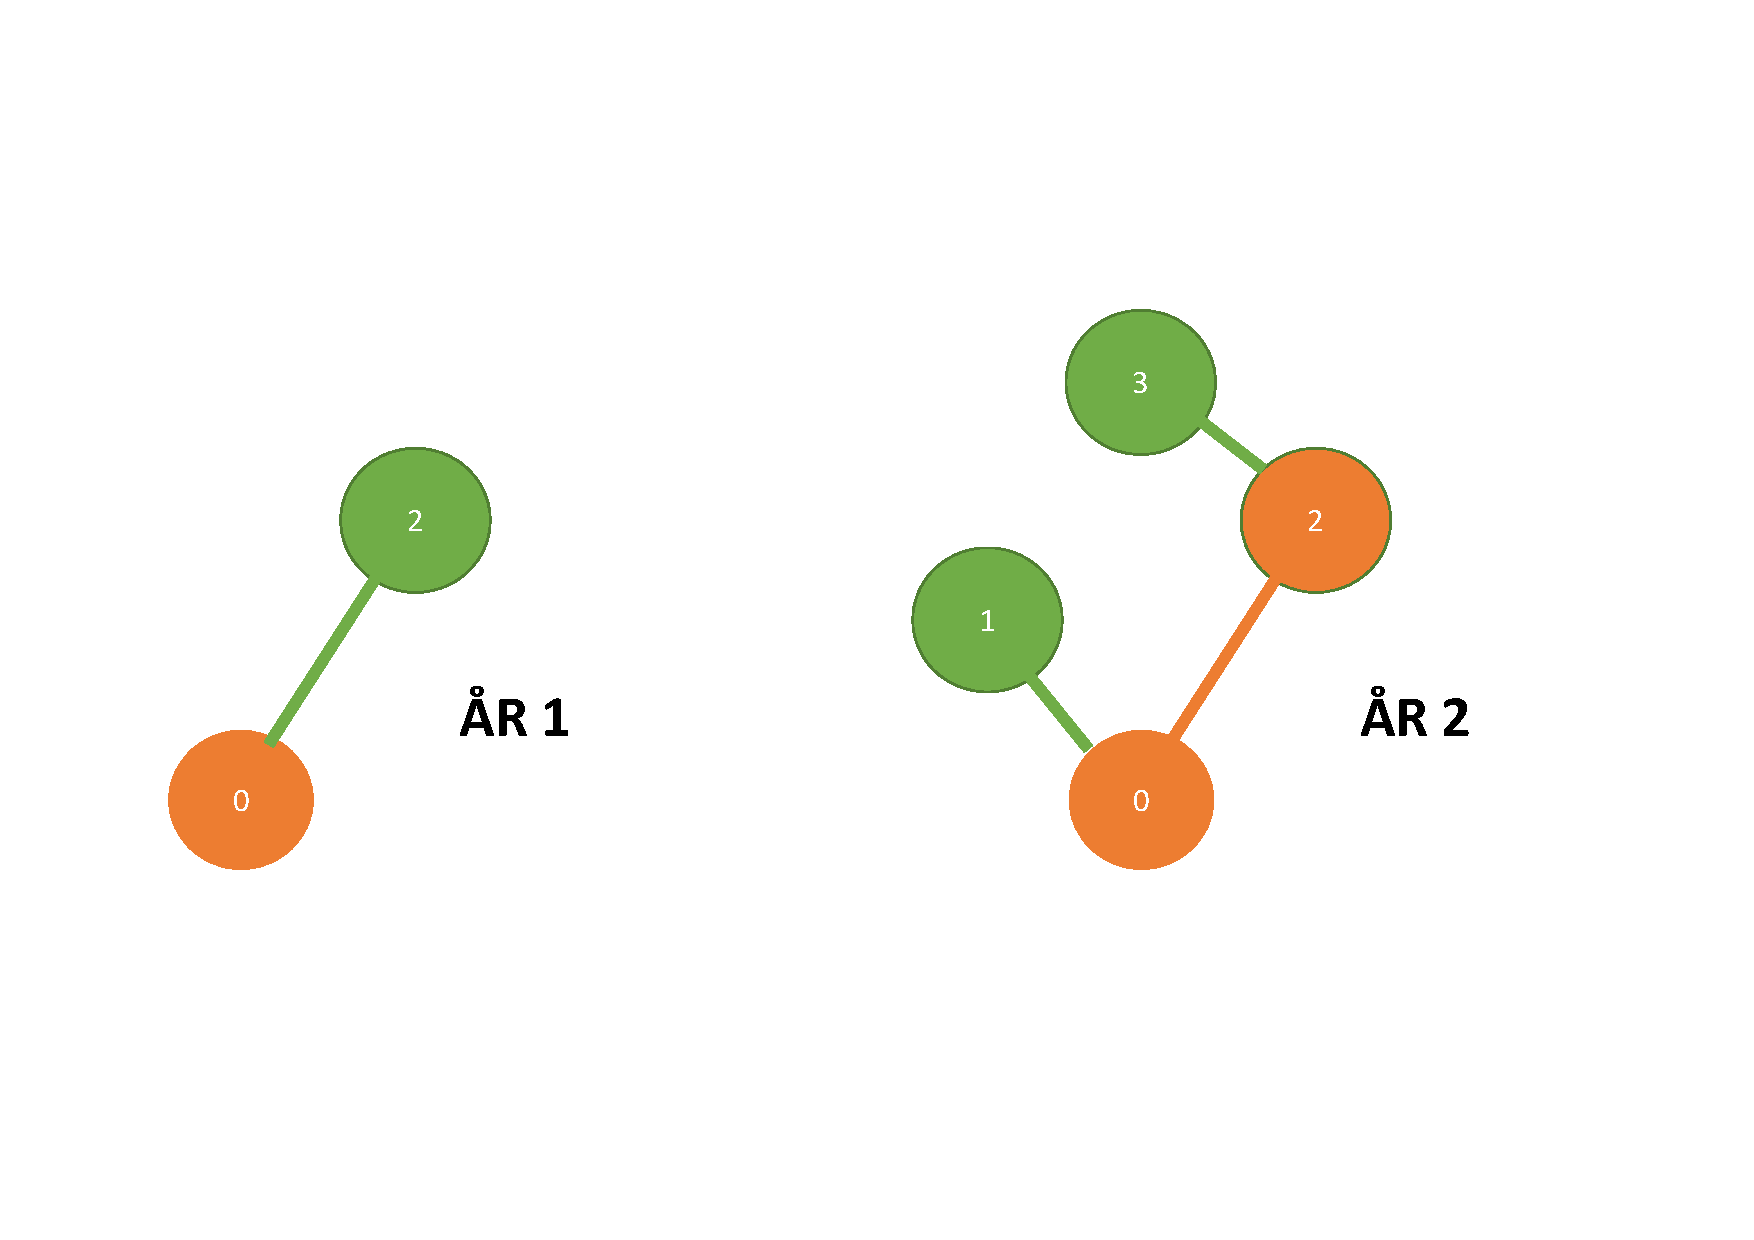
\includegraphics[width=0.5\textwidth]{Bonsai_tree}
\caption{One of the two ways to grow the bonsai tree in the first sample in two years.}
\end{figure}
